\chapter{Program expectations}
The goal of this project is to make a short read alignment software using \gls{ncbi}\slash\gls{blast}.
Before writing it, we need to understand precisely what is expected of it.
This is what we propose to do in this chapter.


\section{Short reads}
\label{sec:shortReads}
\gls{ngs} sequencers usually output their results in fastQ file(s).
FastQs are text files containing records for each read generated by the sequencer.

\begin{SCfigure}[4][h]
\captionsetup{singlelinecheck=off}
\caption[FastQ~format.]{
    A record in a fastQ file is composed of four lines:
    \vspace{1.5ex}
    \begin{itemize}
        \item Read identification preceded by `@',
        \vspace{1.5ex}
        \item \gls{dna} sequence,
        \vspace{1.5ex}
        \item Separator (+),
        \vspace{1.5ex}
        \item Read sequencing quality.
        \vspace{1.5ex}
    \end{itemize}}
\label{fig:fastqExample}
\begin{minipage}{0.3\textwidth}
\begin{minipage}{0.66\textwidth}
\begin{lstlisting}[basicstyle=\ttfamily\small,frameround=ftft,frame=trBL]
@sequenceID.1
ATATCGAT
+
!8ACC@FG
@sequenceID.2
(...)
\end{lstlisting}
\end{minipage}
\end{minipage}
\end{SCfigure}

The read quality is composed of symbols representing the sequencing quality of each base.
This string and the \gls{dna} sequence should have the same length.

As we have seen in section~\ref{sec:ngs}, sequencing can be done in a single-end or paired-end fashion.
If the data is single-end, there should only be one fastQ file.
If the data is paired-end, there are two possibilities:
\begin{itemize}
    \item Two fastQ files are generated, one for each strand of the sequence;
    \item The sequences of the two strands are interleaved in one fastQ file.
\end{itemize}

An example of paired-end fastQ files is represented in figure~\ref{fig:pairedFastq}.

The program is expected to use fastQ files as an input and analyze them properly according to the type of sequencing used (single-end, paired-end or paired-end with interleaved data).

\begin{figure}[H]
\lstset{
    basicstyle=\ttfamily\small,
    frameround=ftft,
    frame=trBL}
\newcolumntype{P}{>{\centering}p{0.3\textwidth}}
\begin{tabular}{P P || P}
\emph{FastQ1} & \emph{FastQ2} & \emph{Interleaved}\tabularnewline
\begin{minipage}[t]{0.2\textwidth}
\begin{lstlisting}
@sequenceID.1
ATATCGAT
+
!8ACC@FG
@sequenceID.2
(...)
\end{lstlisting}
\end{minipage}
&
\begin{minipage}[t]{0.2\textwidth}
\begin{lstlisting}
@sequenceID.1
AGATAGAG
+
!8A@CGGE
@sequenceID.2
(...)
\end{lstlisting}
\end{minipage}
&
\begin{minipage}[t]{0.2\textwidth}
\begin{lstlisting}
@sequenceID.1
ATATCGAT
+
!8ACC@FG
@sequenceID.1
AGATAGAG
+
!8A@CGGE
@sequenceID.2
(...)
@sequenceID.2
(...)
\end{lstlisting}
\end{minipage}
\end{tabular}
\caption{Paired-end fastQ.}
\label{fig:pairedFastq}
\end{figure}


\section{BLAST}
The project states that the alignment must be done with \gls{ncbi}\slash\gls{blast}.
Since we want the results to be directly available as an input of the program, we have decided to use the local version of \gls{blast} (BLAST\texttt{+}).
BLAST\texttt{+} is composed of different pieces of software, each able to align a specific type of sequence.
Our goal being the alignment of short reads sequences against a \gls{dna} reference, we chose the tool blastn (Nucleotide \gls{blast}).


\subsection{BLAST input}
\label{subsec:blastinput}
\gls{blast} cannot process fastQ files, the input sequences must be in fasta format.
Fastas are text files containing records for each sequence.

\begin{SCfigure}[4][h]
\captionsetup{singlelinecheck=off}
\caption[Fasta~format.]{
    A record in a fasta file is composed of two lines:
    \vspace{1.5ex}
    \begin{itemize}
        \item Sequence identification preceded by `\textgreater',
        \vspace{1.5ex}
        \item \gls{dna} sequence.
        \vspace{2.3ex}
    \end{itemize}}
\label{fig:fastaExample}
\begin{minipage}{0.3\textwidth}
\begin{minipage}{0.66\textwidth}
\begin{lstlisting}[basicstyle=\ttfamily\small,frameround=ftft,frame=trBL]
>sequenceID.1
ATATCGAT
>sequenceID.2
(...)
\end{lstlisting}
\end{minipage}
\end{minipage}
\end{SCfigure}

The software is expected to convert and merge fastQ files into a fasta file for \gls{blast} input.


\subsection{BLAST output}
Since the last version of BLAST\texttt{+} (2.2.31), \gls{blast} has 14 different outputs. There is also a 15\textsuperscript{th} undocumented one we will discuss in the general conclusion (page~\pageref{ch:conclusion}).
In order to get the maximum of information about the alignments, \gls{xml} output was chosen (\texttt{outfmt~5}).

Figure~\ref{fig:xmlExample} shows an example of a partial \gls{blast} \gls{xml} output.

\begin{figure}[h!]
\lstset{
    language=XML,
    basicstyle=\ttfamily\footnotesize,
    breaklines=true,
    escapeinside={(*@}{@*)},
    moredelim=[s][\color{Green}]{<}{>},
    frameround=ftft,
    frame=trBL}
\begin{lstlisting}
(...)
<Iteration>
  <Iteration_iter-num>3</Iteration_iter-num>
  <Iteration_query-ID>Query_3</Iteration_query-ID>
  <Iteration_query-def>ERR656485.2</Iteration_query-def>
  <Iteration_query-len>300</Iteration_query-len>
<Iteration_hits>
<Hit>
  <Hit_num>1</Hit_num>
  <Hit_id>gnl|BL_ORD_ID|0</Hit_id>
  <Hit_def>gi|9629357|ref|NC_001802.1| Human immunodeficiency virus 1, complete genome</Hit_def>
  <Hit_accession>0</Hit_accession>
  <Hit_len>9181</Hit_len>
  <Hit_hsps>
    <Hsp>
      <Hsp_num>1</Hsp_num>
      <Hsp_bit-score>148.852</Hsp_bit-score>
      <Hsp_score>80</Hsp_score>
      <Hsp_evalue>4.07002e-39</Hsp_evalue>
      <Hsp_query-from>2</Hsp_query-from>
      <Hsp_query-to>120</Hsp_query-to>
      <Hsp_hit-from>833</Hsp_hit-from>
      <Hsp_hit-to>715</Hsp_hit-to>
      <Hsp_query-frame>1</Hsp_query-frame>
      <Hsp_hit-frame>-1</Hsp_hit-frame>
      <Hsp_identity>106</Hsp_identity>
      <Hsp_positive>106</Hsp_positive>
      <Hsp_gaps>0</Hsp_gaps>
      <Hsp_align-len>119</Hsp_align-len>
      <Hsp_qseq>TGGGCTAAAGGCCTTTTCCTCTATTACTTTTACCCATGCATTTAAAGTTCTAGGTGACATGGCCTGGTG(*@@*)TACCATTTGCCCTTGGAGATTTTGCACTATAGGATAATTTTGACTGACCT</Hsp_qseq>
      <Hsp_hseq>TGGGCTGAAAGCCTTCTCTTCTACTACTTTTACCCATGCATTTAAAGTTCTAGGTGATATGGCCTGATG(*@@*)TACCATTTGCCCCTGGATGTTCTGCACTATAGGGTAATTTTGGCTGACCT</Hsp_hseq>
      <Hsp_midline>|||||| || ||||| || |||| ||||||||||||||||||||||||||||||||| |||||||| |||||||||||||| ||||  || ||||||||||| |||||||| |||||||
      </Hsp_midline>
    </Hsp>
(...)
\end{lstlisting}
\caption{\acrshort{blast} \acrshort{xml} output.}
\label{fig:xmlExample}
\end{figure}

The software is expected to extract the data from a \gls{blast} \gls{xml} output file.


\section{Output}
\label{sec:samoutput}
Popular downstream analysis software such as \href{http://www.htslib.org/}{SAMtools}, \href{https://www.broadinstitute.org/gatk/}{GATK} or \href{https://www.broadinstitute.org/igv/}{IGV} use the standard \gls{sam} or its binary counterpart (BAM).
It is defined in the \gls{sam} format specification~\cite{samspec}.
\gls{sam} is a text-based file containing two parts described below.
\begin{itemize}
    \item Header section:
    \begin{itemize}
        \item @HD: Header line: \gls{sam} format version and sorting order of alignments;
        \item @SQ: Reference sequence dictionary: reference sequence name and its length;
        \item @RG: Read group: read group identifier and sample name;
        \item @PG: Program: aligner identifier, name, version and command-line used.
    \end{itemize}
    \item Alignment section, composed of at least 11 elements:
    \begin{enumerate}
        \item QNAME: Read name;
        \item FLAG: Bitwise flag used to categorize the read according to its alignment on the reference;
        \item RNAME: Name of the reference on which the read is mapped;
        \item POS: Position on the reference at which the read is mapped;
        \item MAPQ: Mapping quality of the read;
        \item CIGAR: \gls{cigar} is string representation of the alignment.
        `=' represents a match, `X' a mismatch, `I' an insertion, `D' a deletion, `N' a long deletion, `S' a soft-clipped base, `H' a hard-clipped one.
        `M' can be used to represent either a match or a mismatch.
        A base is soft-clipped if it does not take part in the alignment but the base is still shown in the sequence.
        Hard-clipped bases differ by the fact that they are not shown in the sequence.
        In both cases, they can only be encountered at the ends of the reads.
        In the \gls{cigar} string, the number before the symbol represents the number of times the symbol is encountered before a different one occurs;
        Example: \texttt{1S3=2X1I} means that the alignment begins with a soft-clipped base, followed by three matches, two mismatches and an insertion.
        \item RNEXT: Name of the reference on which the read's mate is mapped;
        \item PNEXT: Position on the reference at which the read's mate is mapped;
        \item TLEN: Distance on the reference between the 5'~end of the read and the 5'~end of its mate;
        \item SEQ: Sequence of the read;
        \item QUAL: Sequencing quality of the read;
        \item Metadata: Optional supplementary information on the read.
    \end{enumerate}   
\end{itemize}

Figure~\ref{fig:samBWA} shows an example of a \gls{sam} file generated by \gls{bwa}.

The software is expected to produce a \gls{sam} file compatible with downstream softwares.


\section{Implementation language}
\gls{blast} is known to be slower than more recent aligners.
To avoid slowing down further the mapping, an implementation in a compiled language would be preferred.
The program is expected to be able to read gzipped formatted files (fastQ files are usually compressed) and to parse an \gls{xml} file.
Very well known C libraries can be used to that goal: \href{http://www.zlib.net/}{zlib} and \href{http://www.xmlsoft.org/}{libxml2}.
To maximize speed, the program will be implemented in C.

Based on these expectations, we devised a general outline of the program to implement (fig~\ref{fig:generalOutline}).

\begin{figure}
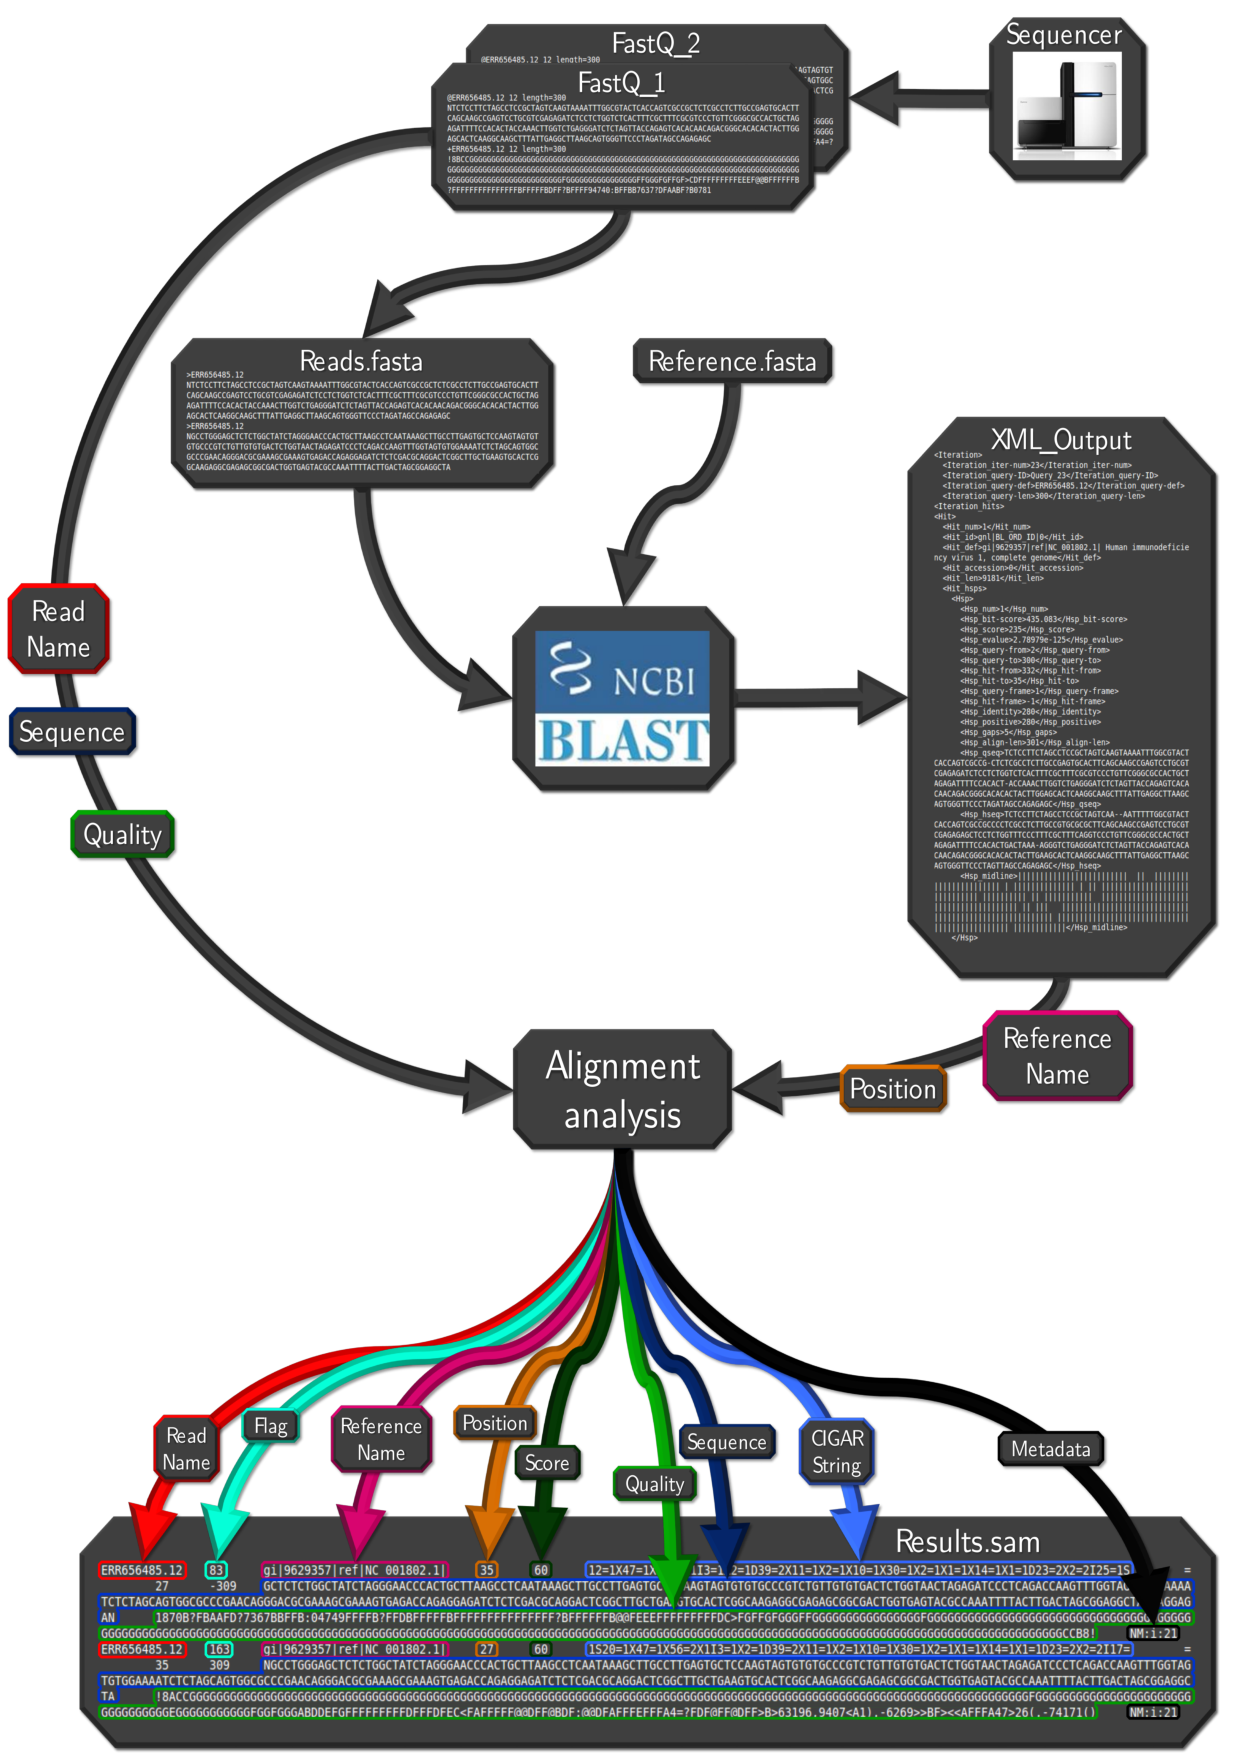
\includegraphics[scale=0.75]{img/generalOutline}
\caption{General outline of the program.}
\label{fig:generalOutline}
\end{figure}
